\documentclass[tikz,border=2pt]{standalone}
\usepackage{amsmath}
\usepackage{pgfplots}
\pgfplotsset{compat=1.18}

\begin{document}
% The graph of |x|: two half-lines meeting at the origin; |−2| = 2 is the distance from −2 to 0.
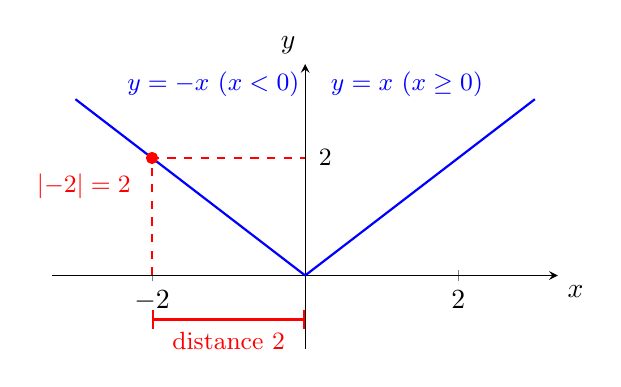
\begin{tikzpicture}
	\begin{axis}[
		axis lines=middle,
		xmin=-3.3, xmax=3.3,
		ymin=-1.25, ymax=3.6,
		xtick={-2,2}, ytick=\empty,
		xlabel={$x$}, ylabel={$y$},
		xlabel style={below right}, ylabel style={above left},
		samples=2, clip=false,
		width=8cm, height=5.2cm
		]
		\addplot[thick, blue, domain=-3:0] {-x};
		\addplot[thick, blue, domain=0:3] {x};
		\node[blue, anchor=west, font=\small] at (axis cs:-2.45,3.25) {$y=-x$ ($x<0$)};
		\node[blue, anchor=east, font=\small] at (axis cs:2.45,3.25) {$y=x$ ($x\ge 0$)};
		\draw[dashed, red] (axis cs:-2,0) -- (axis cs:-2,2) -- (axis cs:0,2);
		\addplot[only marks, mark=*, red] coordinates {(-2,2)};
		\node[anchor=west, font=\small] at (axis cs:0.05,2) {$2$};
		\node[red, anchor=north east, font=\small] at (axis cs:-2.15,1.9) {$|{-2}|=2$};
		\draw[red, thick, |-|] (axis cs:-2,-0.75) -- (axis cs:0,-0.75);
		\node[red, anchor=north, font=\small] at (axis cs:-1,-0.8) {distance $2$};
	\end{axis}
\end{tikzpicture}
\end{document}
